\documentclass[11pt,a4paper]{article}

% Packages
\usepackage[utf8]{inputenc}
\usepackage[spanish, es-tabla, es-lcroman]{babel}
\usepackage{caption}
\usepackage{listings}
\usepackage{adjustbox}
\usepackage{amssymb, amsmath, amsthm}
\usepackage[margin=1in]{geometry}
\usepackage[shortlabels]{enumitem}
\usepackage{xcolor}
\usepackage{soul}
\usepackage{listings}
\usepackage{graphicx}
\usepackage{float}

% Meta
\title{Práctica 1: Estudio de la eficiencia}
\author{José Antonio Álvarez Ocete}
\date{\today}

% Custom
\providecommand{\abs}[1]{\lvert#1\rvert}
\setlength\parindent{0pt}
\definecolor{Light}{gray}{.90}
\newcommand\ddfrac[2]{\frac{\displaystyle #1}{\displaystyle #2}}

% Listings
\lstset{literate=   % listings config
  {á}{{\'a}}1 {é}{{\'e}}1 {í}{{\'i}}1 {ó}{{\'o}}1 {ú}{{\'u}}1
  {Á}{{\'A}}1 {É}{{\'E}}1 {Í}{{\'I}}1 {Ó}{{\'O}}1 {Ú}{{\'U}}1
  {à}{{\`a}}1 {è}{{\`e}}1 {ì}{{\`i}}1 {ò}{{\`o}}1 {ù}{{\`u}}1
  {À}{{\`A}}1 {È}{{\'E}}1 {Ì}{{\`I}}1 {Ò}{{\`O}}1 {Ù}{{\`U}}1
  {ä}{{\"a}}1 {ë}{{\"e}}1 {ï}{{\"i}}1 {ö}{{\"o}}1 {ü}{{\"u}}1
  {Ä}{{\"A}}1 {Ë}{{\"E}}1 {Ï}{{\"I}}1 {Ö}{{\"O}}1 {Ü}{{\"U}}1
  {â}{{\^a}}1 {ê}{{\^e}}1 {î}{{\^i}}1 {ô}{{\^o}}1 {û}{{\^u}}1
  {Â}{{\^A}}1 {Ê}{{\^E}}1 {Î}{{\^I}}1 {Ô}{{\^O}}1 {Û}{{\^U}}1
  {œ}{{\oe}}1 {Œ}{{\OE}}1 {æ}{{\ae}}1 {Æ}{{\AE}}1 {ß}{{\ss}}1
  {ű}{{\H{u}}}1 {Ű}{{\H{U}}}1 {ő}{{\H{o}}}1 {Ő}{{\H{O}}}1
  {ç}{{\c c}}1 {Ç}{{\c C}}1 {ø}{{\o}}1 {å}{{\r a}}1 {Å}{{\r A}}1
  {€}{{\EUR}}1 {£}{{\pounds}}1 {ñ}{{\~{n}}}1
}

\lstset{    %listings config
	language=C++,
	belowcaptionskip=1\baselineskip,
	breaklines=true,
	frame=L,
	xleftmargin=0.1in,
	%otherkeywords={},
	showstringspaces=false,
	backgroundcolor=\color{white},
	basicstyle=\footnotesize\ttfamily,
	keywordstyle=\bfseries\color{purple!90!black},
	commentstyle=\itshape\color{gray!85!},
	identifierstyle=\color{blue!80!black},
	stringstyle=\color{green!60!black},
}

\begin{document}

\maketitle

\section{Introducción}

En este práctica realizaremos un estudio de la eficiencia tanto empírica como híbrida de los algoritmos propuestos en el guión de prácticas. Siguiendo este guión, realizaremos distintas gráficas mostrando el trabajo realizado y expondremos diversos resultados.

Adjunto a esta memoria entrego los datos tomados así como las gráficas generadas a partir de los mismos.

\section{Informe de la eficiencia}

Los algoritmos propuestos para el estudio de la eficiencia son los siguientes:

\begin{table}[H]
	\centering
	\caption{Algoritmos a estudiar.}
	\label{my-label}
	\begin{tabular}{ll}
		Algoritmo & Eficiencia   \\
		burbuja   & $O(n^2)$     \\
		inserción & $O(n^2)$     \\
		selección & $O(n^2)$     \\
		mergesort & $O(n log n)$ \\
		quicksort & $O(n log n)$ \\
		heapsort  & $O(n log n)$ \\
		floyd     & $O(n^3)$     \\
		hanoi     & $O(2^n)$      
	\end{tabular}
\end{table}

\subsection{Algoritmos de orden cuadrático}

En primer lugar realizamos un estudio teórico de la eficiencia. Como se vió en el guión de prácticas, la eficiencia teórica de el algoritmo \emph{burbuja} es de:

$$\frac{a}{2} n^2 - \frac{3a}{2} n + a \in O(n^2)$$

Donde $a$ es una constante que acota el interior del bucle.

Repetimos un proceso análogo al realizado para el algóritmo de burbuja estudiando \textbf{selección} para el siguiente código:

\newpage

\begin{lstlisting}
static void seleccion_lims(int T[], int inicial, int final) {
	int i, j, indice_menor;
	int menor, aux;
	for (i = inicial; i < final - 1; i++) {
		indice_menor = i;
		menor = T[i];
		for (j = i; j < final; j++) {
			if (T[j] < menor) {
				indice_menor = j;
				menor = T[j];
			}
		}
		aux = T[i];
		T[i] = T[indice_menor];
		T[indice_menor] = aux;
	};
}
\end{lstlisting}

Acotando de nuevo el interior del bucle por una constante $a$, denotando $n$ por el tamaño del vector y a partir de los dos bucles obtenemos fácilemente:

$$\sum_{i=0}^{n-1} \sum_{j=i}^{n} a = a \cdot \sum_{i=0}^{n-1} n - i + 1 = a \cdot ( \sum_{i=0}^{n-1} (n + 1) - \sum_{i=0}^{n-1}(i) ) =  $$
$$ = a \cdot ((n+1)(n-1) - \frac{(n-1)(n)}{2}) = a \cdot (\frac{n^2}{2} - \frac{n}{2} - 1) \in O(n^2)$$

Para el caso de \textbf{inserción} tenemos el siguiente algoritmo:

\begin{lstlisting}
static void insercion_lims(int T[], int inicial, int final)
{
	int i, j;
	int aux;
	for (i = inicial + 1; i < final; i++) {
		j = i;
		while ((T[j] < T[j-1]) && (j > 0)) {
			aux = T[j];
			T[j] = T[j-1];
			T[j-1] = aux;
			j--;
		};
	};
}
\end{lstlisting}

Manteniendo la notación utilizado y utilizando un razonamiento similiar al anterior obtenemos:

$$\sum_{i=0}^{n} \sum_{j=i}^{n} a = ... = a \cdot (\frac{n^2}{2} + 2n) \in O(n^2)$$

Realizado el estudio teórico sobre los tres algoritmos, ejecutamos y utilizamos \emph{gnuplot} para obtener un ajuste de los datos obtenidos. Representamos ahora el ajuste junto los datos. 

\begin{figure}[H]
	\centering
	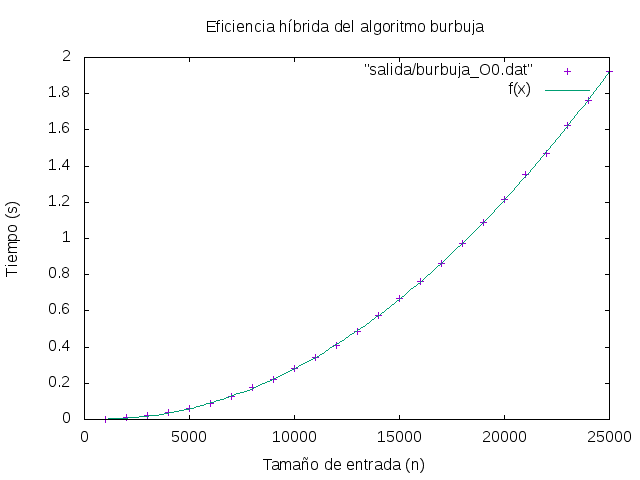
\includegraphics[width=0.8\textwidth]{../plots/burbuja_O0_fit.png}
	\caption{Eficiencia híbridia del algoritmo $burbuja$.}
\end{figure}

\begin{figure}[H]
	\centering
	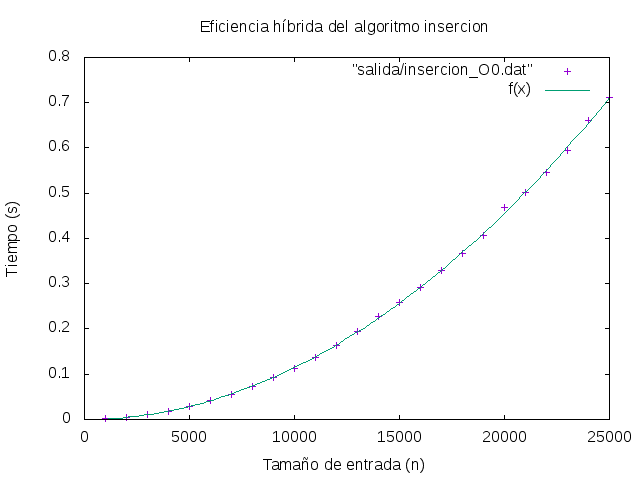
\includegraphics[width=0.8\textwidth]{../plots/insercion_O0_fit.png}
	\caption{Eficiencia híbridia del algoritmo $insercion$.}
\end{figure}

\begin{figure}[H]
	\centering
	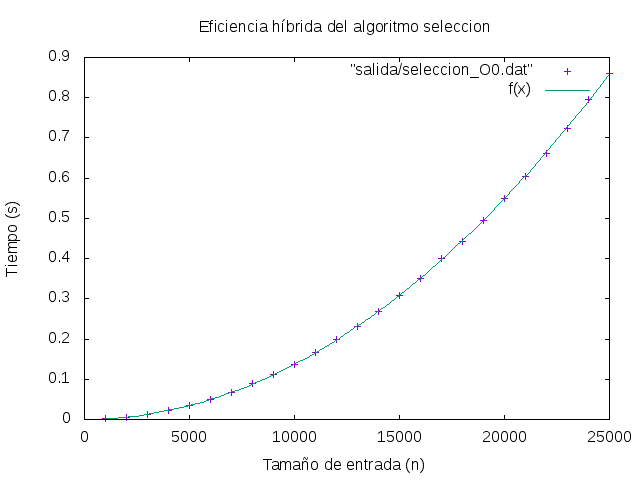
\includegraphics[width=0.8\textwidth]{../plots/seleccion_O0_fit.png}
	\caption{Eficiencia híbridia del algoritmo $seleccion$.}
\end{figure}

Veamos finalmente una comparativa de los tres algoritmos.

\begin{figure}[H]
	\centering
	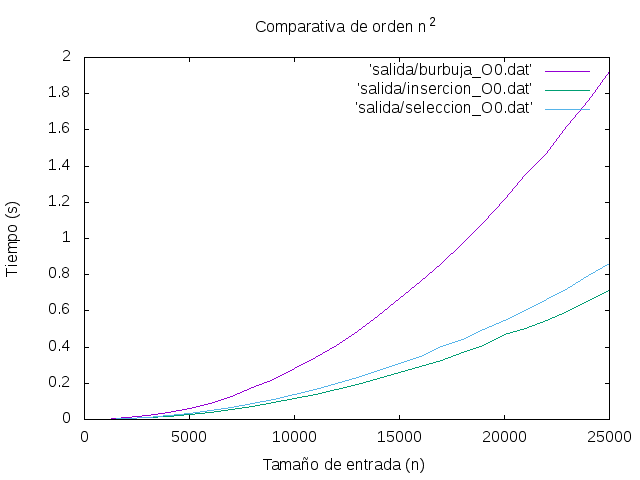
\includegraphics[width=0.8\textwidth]{../plots/cuadraticos_O0.png}
	\caption{Comparativa de algoritmos de orden cuadrático.}
\end{figure}

\subsection{Algoritmos de orden n - logarítimico}

De nuevo comencemos realizando un estudio teórico. Como se vió en el guión de prácticas, la eficiencia teórica de el algoritmo \emph{mergesort} es de:

$$c_1n + c_2nlog_2(n) \in O(nlog_2(n))$$

Para el caso de \textbf{heapsort} tenemos el siguiente algoritmo:

\begin{lstlisting}
static void heapsort(int T[], int num_elem) {
	int i;
	for (i = num_elem/2; i >= 0; i--)
		reajustar(T, num_elem, i);
	for (i = num_elem - 1; i >= 1; i--) {
		int aux = T[0];
		T[0] = T[i];
		T[i] = aux;
		reajustar(T, i, 0);
	}
}

static void reajustar(int T[], int num_elem, int k) {
	int j;
	int v;
	v = T[k];
	bool esAPO = false;
	while ((k < num_elem/2) && !esAPO) {
		j = k + k + 1;
		if ((j < (num_elem - 1)) && (T[j] < T[j+1]))
			j++;
		if (v >= T[j])
			esAPO = true;
		T[k] = T[j];
		k = j;
	}
	T[k] = v;
}
\end{lstlisting}

Estudiaremos en primer lugar la eficiencia de la función $Reajustar(k)$ que denotaremos por $R(k)$. Si nos fijamos en la primera línea del bucle, en cada iteración multiplicamos $k \cdot 2$. Por lo tanto, si acotamos el interior del bucle por una constance $c_1$ y $ t = n-k$:

$$R(n-k) = R(\frac{n-k}{2}) + c_1 \leftrightarrow R(t) = R(\frac{t}{2}) + c_1$$

Aplicando el cambio de variable $t = 2^m \leftrightarrow log_2 t = m$:

$$R(2^m) = R(2^{m-1}) + c_1$$

Denotando $R(2^m) = X_m$ obtenemos una ecuación en recurrencia:

$$X_m = X_{m-1} + c_1$$

Cuya solución es:

$$X_m = c_2 + c_1 * m$$

Donde $c_2$ es otra constance. Deshaciendo el cambio de variable obtenemos finalmente:

$$R(2^m) = R(t) = c_2 + c_1 * log_2(t) \in O(log(n))$$

A partir de la eficiencia de la función \textbf{Reajustar} es relativamente sencillo obtener la del algoritmo completo:

$$\sum_{i=0}^{n/2} R(i) + \sum_{i=1}^{n-1} (R(i) + c_3) $$

Como el logarítmo es una función creciente, acotamos los valores interiores de los bucles por el mayor valor alcanzado:

$$\sum_{i=0}^{n/2} R(i) + \sum_{i=1}^{n-1} (R(i) + c_3) \leq \sum_{i=0}^{n/2} R(n/2) + \sum_{i=1}^{n-1} (R(n-1) + c_3) = $$

$$= (n/2) \cdot R(n/2 + 1) + (n-1) \cdot R(n - 1) + c_3(n-1) = $$

$$= (n/2) \cdot R(n/2 + 1) + (n-1) \cdot R(n - 1) + c_3(n-1)$$

Como el orden de eficiencia de \textbf{Reajustar} es de $O(log(n))$, podemos concluir que el algoritmo tiene una eficiencia de $O(nlog(n))$

Realizado el estudio teórico sobre los tres algoritmos, ejecutamos y utilizamos \emph{gnuplot} para obtener un ajuste de los datos obtenidos. Representamos ahora el ajuste junto los datos. 

\begin{figure}[H]
	\centering
	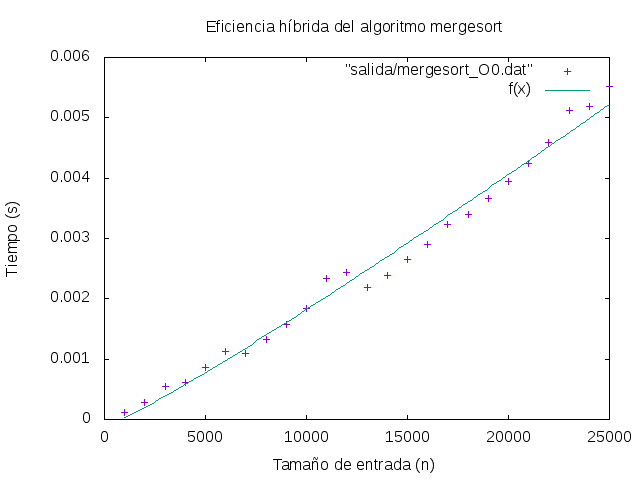
\includegraphics[width=0.8\textwidth]{../plots/mergesort_O0_fit.png}
	\caption{Eficiencia híbridia del algoritmo $mergesort$.}
\end{figure}

\begin{figure}[H]
	\centering
	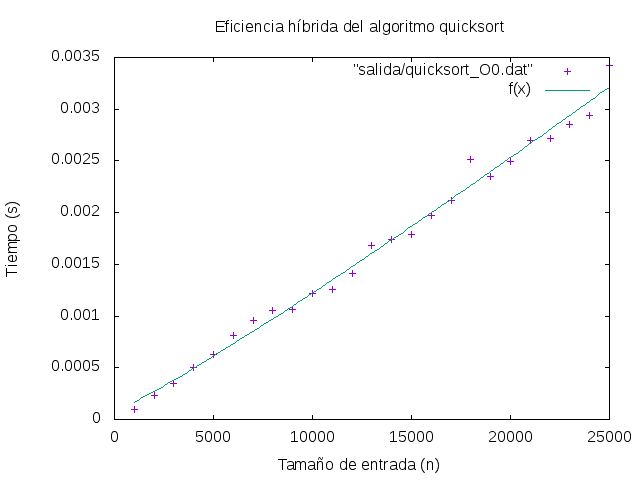
\includegraphics[width=0.8\textwidth]{../plots/quicksort_O0_fit.png}
	\caption{Eficiencia híbridia del algoritmo $quicksort$.}
\end{figure}

\begin{figure}[H]
	\centering
	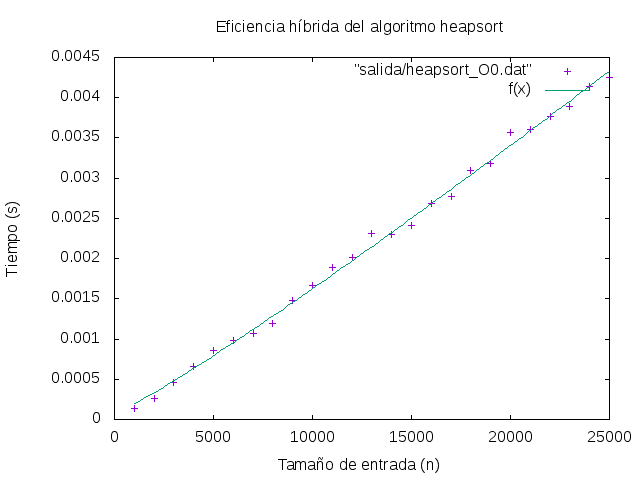
\includegraphics[width=0.8\textwidth]{../plots/heapsort_O0_fit.png}
	\caption{Eficiencia híbridia del algoritmo $heapsort$.}
\end{figure}

Veamos finalmente una comparativa de los tres algoritmos.

\begin{figure}[H]
	\centering
	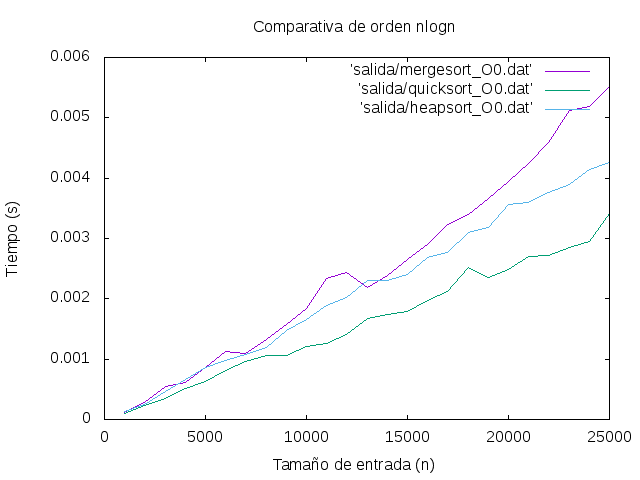
\includegraphics[width=0.8\textwidth]{../plots/logaritmicos_O0.png}
	\caption{Comparativa de algoritmos de orden n-logarítmico.}
\end{figure}

\subsection{Algoritmo de orden cúbico}

Comencemos con el estudio teórico, manteniendo la notación utilizada hasta ahora. He aqui el algoritmo a estudiar, \textbf{floyd}:

\begin{lstlisting}
void Floyd(int **M, int dim) {
	for (int k = 0; k < dim; k++)
		for (int i = 0; i < dim;i++)
			for (int j = 0; j < dim;j++){
				int sum = M[i][k] + M[k][j];    	
				M[i][j] = (M[i][j] > sum) ? sum : M[i][j];
			}
}	     	
\end{lstlisting}

$$\sum_{k=0}^{n} \sum_{i=0}^{n} \sum_{j=0}^{n} a = a n^3 \in O(n^3)$$

Representación de los datos obtenidos junto con su ajuste correspondiente:

\begin{figure}[H]
	\centering
	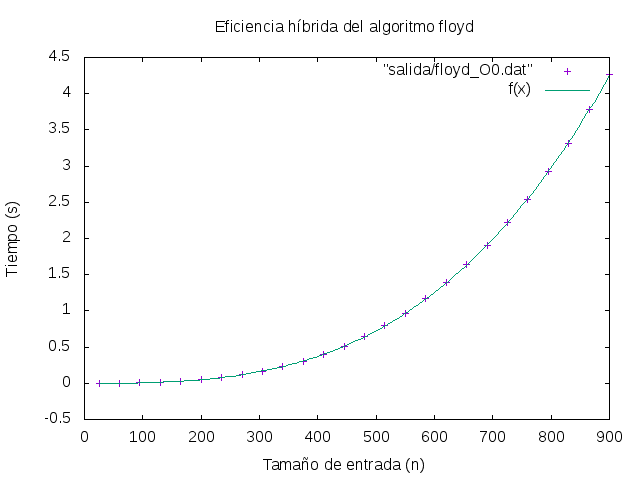
\includegraphics[width=0.8\textwidth]{../plots/floyd_O0_fit.png}
	\caption{Eficiencia híbridia del algoritmo $floyd$.}
\end{figure}

\subsection{Algoritmo de orden exponencial}

Comencemos con el estudio teórico. He aqui el algoritmo a estudiar, \textbf{hanoi}:

\begin{lstlisting}
void hanoi (int M, int i, int j) {
	if (M > 0) {
		hanoi(M-1, i, 6-i-j);
		hanoi (M-1, 6-i-j, j);
	}
}	     	
\end{lstlisting}

Como este algoritmo se llama a si mismo dos veces podemos expresar su eficiencia vara una entrada $n$ como:

$$Hanoi(n) = 2 \cdot Hanoi(n-1)$$

Viendo esta expresión como una ecuación en recurrencias:

$$X_{n+1} = 2 \cdot X_n$$

Esto es una progresión geométrica cuya solución viene expresada por:

$$X_n = C \cdot 2^n \in O(2^n)$$

Donde $C$ es una constante que depende del problema. Una vez finalizado el estudio teórico representamos los datos obtenidos junto con su ajuste correspondiente:

\begin{figure}[H]
	\centering
	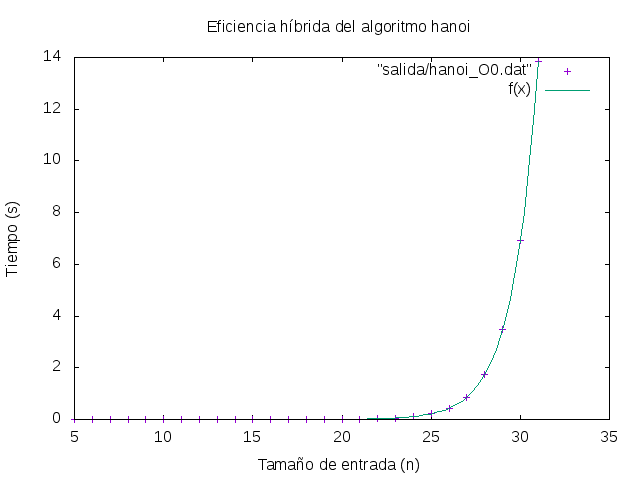
\includegraphics[width=0.8\textwidth]{../plots/hanoi_O0_fit.png}
	\caption{Eficiencia híbridia del algoritmo $hanoi$.}
\end{figure}

\section{Comparativa final}

Veamos finalmente una comparativa de todos los algoritmos utilizados en la práctica.

\begin{figure}[H]
	\centering
	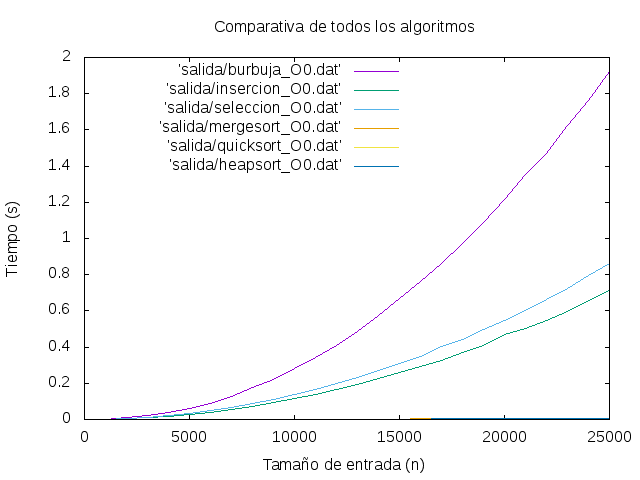
\includegraphics[width=0.8\textwidth]{../plots/todos_ordenacion_O0.png}
	\caption{Eficiencia híbridia del algoritmo $hanoi$.}
\end{figure}

\end{document}